%!TEX root = ../main.tex
\section{Zeitgemäß}
Der Zeitgemäße Design-Entwurf hat zur Aufgabe dem Benutzer eine möglichst bekannte Nutzererfahrung zu bieten. Er soll sich direkt über bekannte Design-Elemente auf der Seite zurechtfinden. 
Jeder Designentwurf in diesem Ansatz verfolgt gleichzeitig den Ansatz des Mobile-First. Demzufolge werden verschiedene Endgeräte in die Überlegungen mit einbezogen.

\subsection{Comprehensive Dummy}
\begin{figure} [hp]
	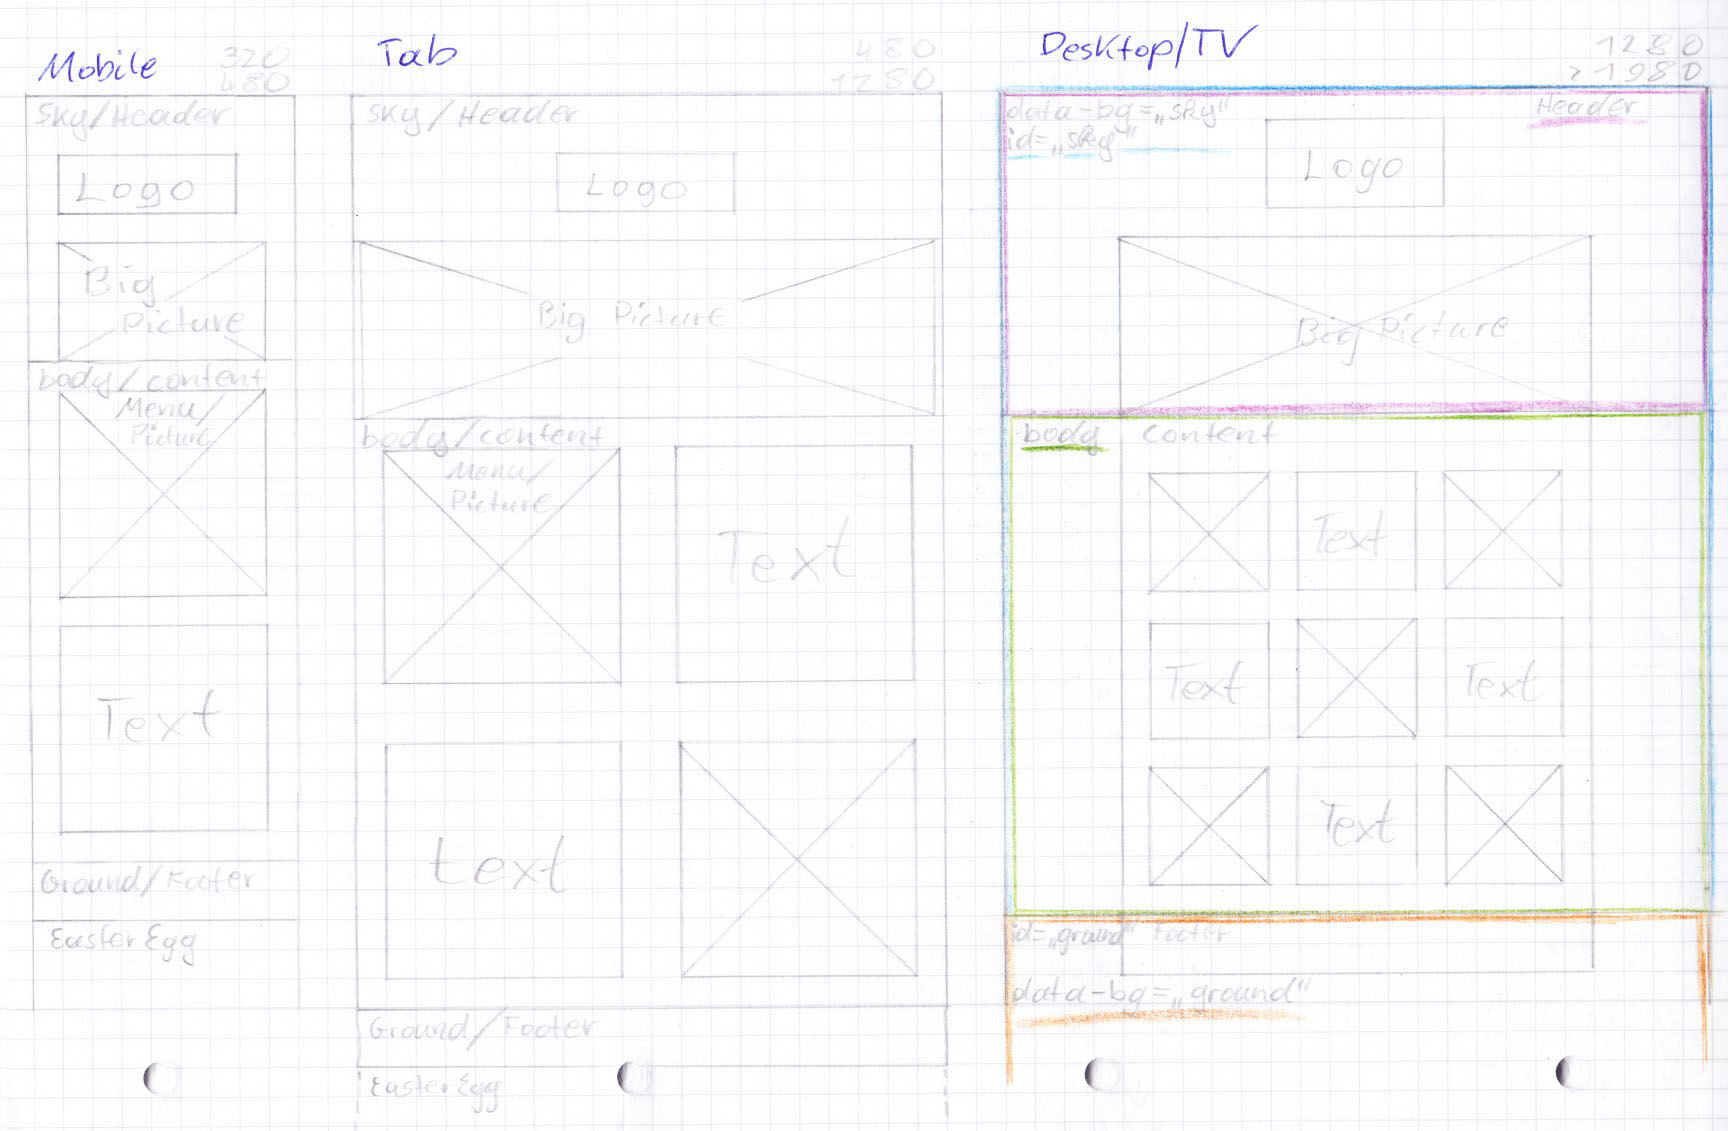
\includegraphics[width=\textwidth]{./img/zeitg_comp1.jpg}
	\caption{Ein erster Entwurf des zeitgemäßen Ansatzes mit Stift und Papier.}
	\label{zeitg:Comp1}
\end{figure}

Die erste Version des Comprehensive Dummy setzt ein Kacheldesign für Inhalts- und Bildblöcke in Form von Fenstern eines Hochhauses um. Wie in Abbildung \ref{zeitg:Comp1} zu sehen ist, wird hier auf ein bekanntes vertikales Layout bestehend aus den drei großen Bereichen, Kopf, Köper und Fußzeile vertraut. In der Kopfzeile soll ein großes Bild die Aufmerksamkeit des Users fangen. Neben dem Logo und einem Himmel als Hintergrund wird ansonsten auf weitere Inhalte im Header verzichtet. Auf mobilen Endgeräten wird noch auf ein einspaltiges Layout gesetzt, welches auf größeren Geräten mehr Spalten erhält um den Platz effektiv zu nutzen. Als designtechnisches Element wird auf Bildschirmen mit genügend Platz ein Whitespace mit Hintergrundgrafik links und rechts der Inhaltsblöcke verwendet.

Nach weiteren Überlegungen entsteht ein weiterer Comprehensive Dummy. Die Entscheidung zu diesem Schritt fußt auf den Überlegungen, dass zum einen eine Navigation in bekannter Weise fehlt und zum anderen das Bild eines Hochhauses nicht zur Zielgruppe der privaten Hauseigentümer passt.
Abbildung \ref{zeitg:Comp2} zeigt einen Ansatz, bei dem sich das Design am Logo orientiert. Auch hier stellt es im Grunde eine abstraktion eines Hauses dar. Diesmal jedoch ist ein Menü direkt am oberen Ende präsent. Ebenso sind die Inhaltsblöcke wieder als Fenster angedeutet.

\begin{figure} [hp]
	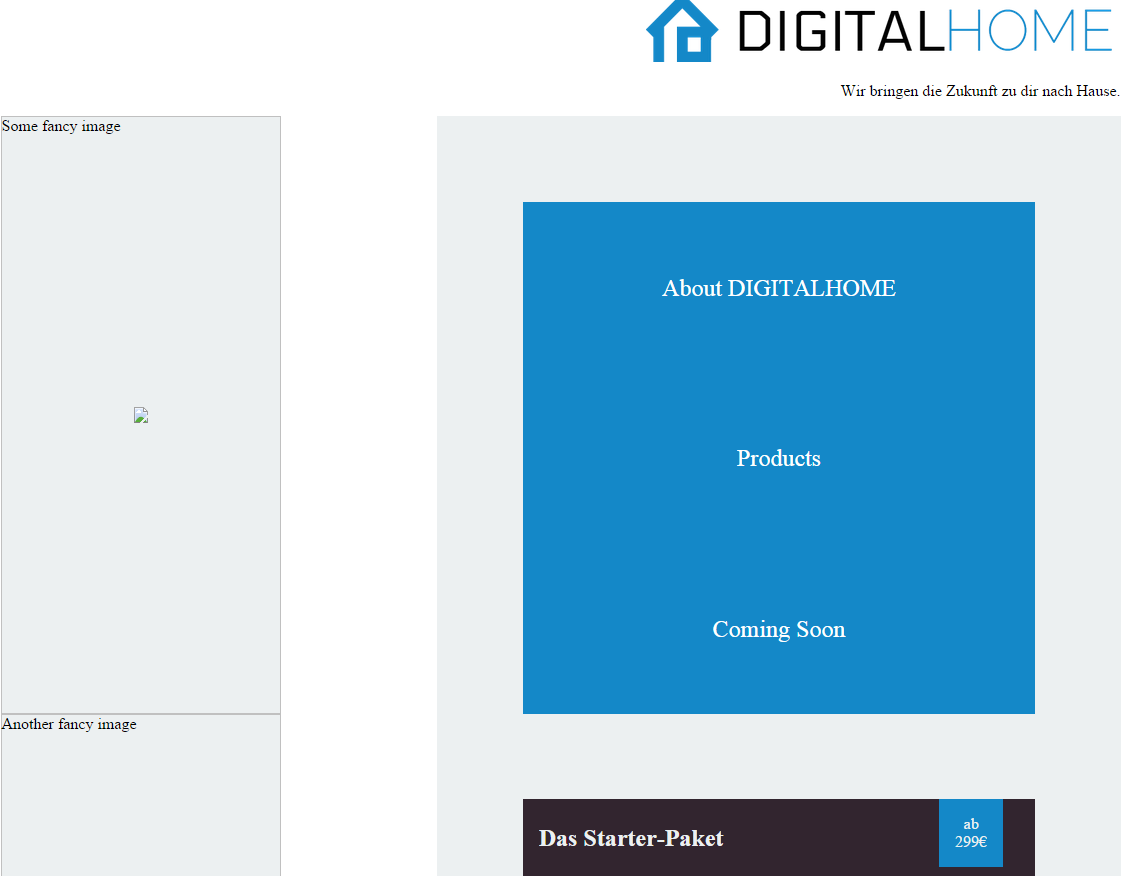
\includegraphics[width=\textwidth]{./img/zeitg_comp2.png}
	\caption{Der zweite Entwurf des zeitgemäßen Ansatzes. Diesmal bereits in HTML und CSS.}
	\label{zeitg:Comp2}
\end{figure}

Letzten Endes ist auch dieses Design nicht vertraut genug und etwas zu minimalistisch. Es folgt der letzte Entwurf, der explizit bekanntere Wege geht (siehe Abbildung \ref{zeitg:Comp3}. Weitere Einzelheiten zur Analyse der Struktur folgt im Kapitel \nameref{zeitg:struktur} auf Seite \pageref{zeitg:struktur}.

\begin{figure} [hp]
	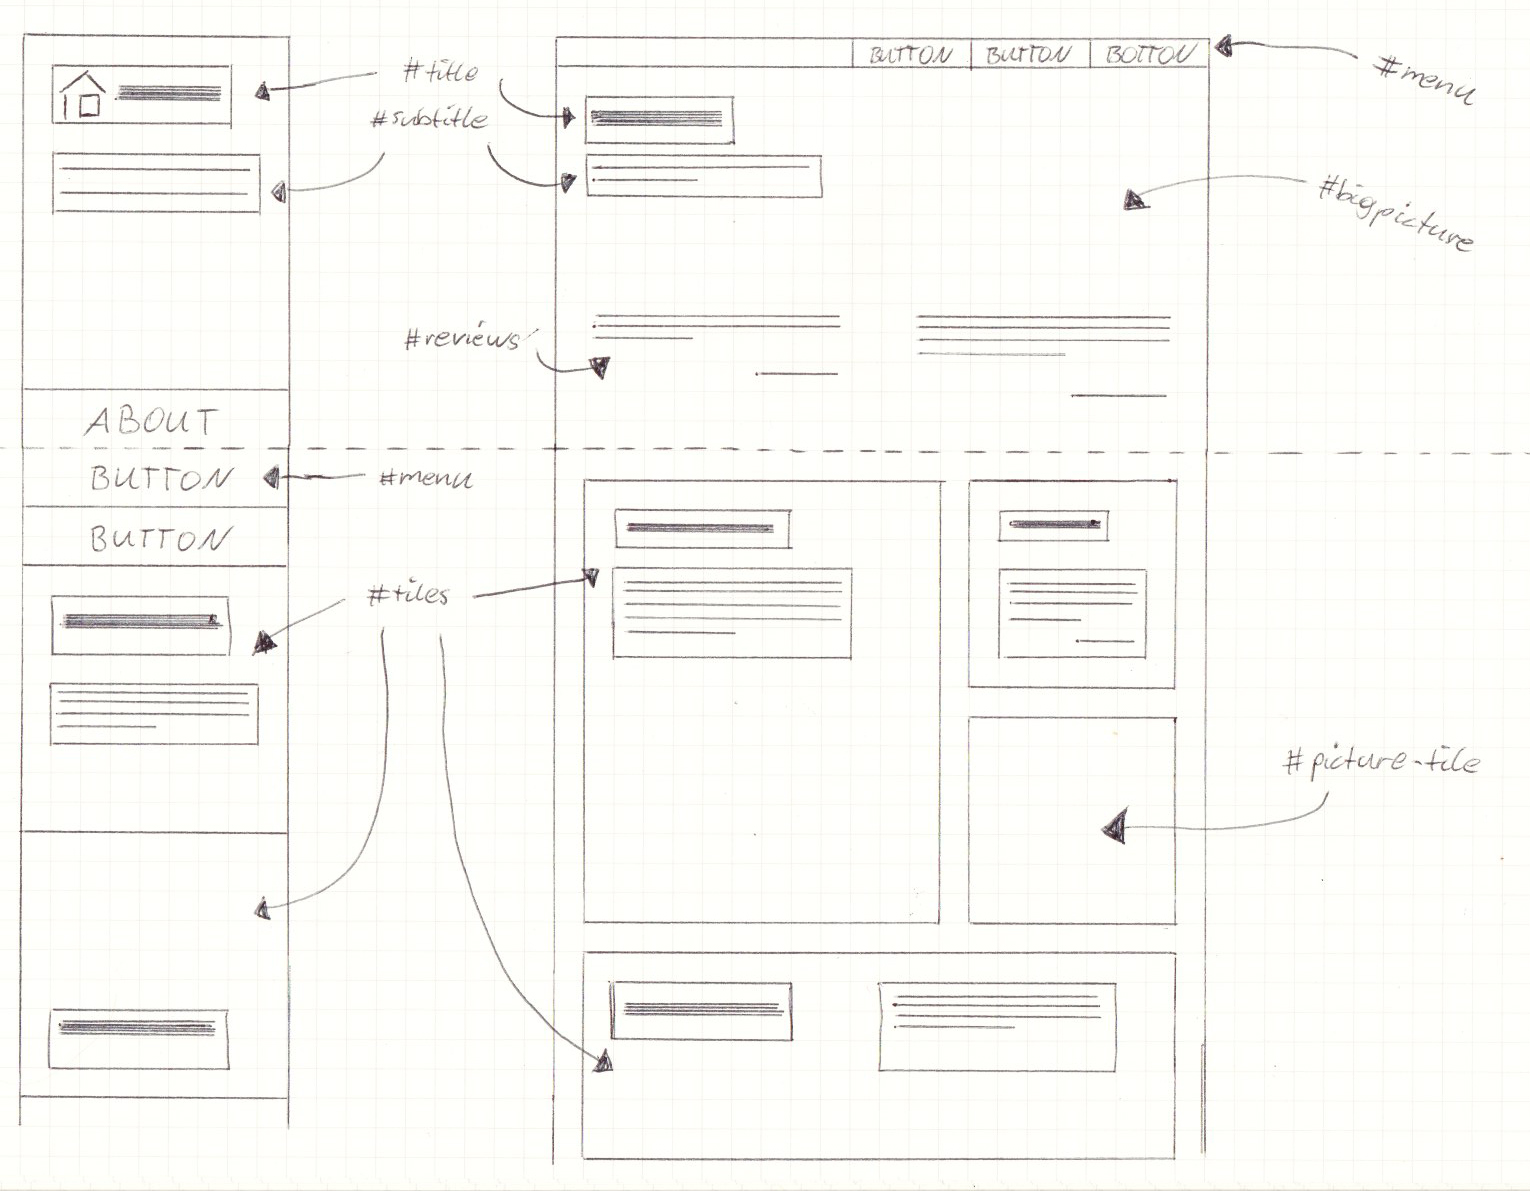
\includegraphics[width=\textwidth]{./img/zeitg_comp3.jpg}
	\caption{Der dritte und letzte Entwurf des zeitgemäßen Ansatzes mit Stift und Papier}
	\label{zeitg:Comp3}
\end{figure}

\subsection{Entwicklungsphase HTML\&CSS}
Die Entwicklung des Markups in HTML stützt sich auf das neue HTML5 und nutzt somit HTML-Tags wie \lstinline{<section>}, \lstinline{<nav>} und \lstinline{<footer>}.
Interessant bzw. speziell ist in diesem Zusammenhang lediglich noch das verwendete Kachel-System, welches eigens für diese Seite entwickelt wurde. Hierbei wurde auf die sog. AM-Modules zurückgegriffen.\footcite[vgl.][]{glen:am} Bei diesem Ansatz definiert man statt CSS-Klassen CSS-Attribute und weißt ihnen die Styles zu. Der Vorteil liegt hierbei im Namespace-Charakter. Der Namespace für die Kacheln lautet \lstinline{[am-Tile]}. Im Codeauszug \ref{code:zeitg:css1} ist zusehen, wie dem Namespace zuerst ein Grundstil vergeben wird und anschließend auf Elemente mit der Eigenschaft \lstinline{~="featured"} weitere Verfeinerungen angewendet werden.

\begin{lstlisting}[caption=AM-Modules zur Definition eines Namespace in CSS., label=code:zeitg:css1]
[am-Tile] {
	width: $column-width;
	padding-bottom: $column-width;
	position: relative;
	margin-bottom: $column-margin;
	margin-left: $column-margin;
	transition: all .3s linear;
	float: left;
}
[am-Tile~="featured"] {
	padding-bottom: 2 * $column-width + $column-margin;
	width: 2 * $column-width + $column-margin;
}
\end{lstlisting}

Desweiteren wird der CSS Code in der Präprozessor-Sprache SCSS geschrieben und anschließend in Valides CSS compiliert. Zu sehen anhand des Codeauszugs \ref{code:zeitg:css2}.

\begin{lstlisting}[caption=Verschachtelung von CSS-Klassen in SCSS., label=code:zeitg:css2]
nav {
	flex-direction: row;
	justify-content: flex-end;
	flex-flow: row wrap;
	& > a {
		padding: 0 2.5em;
		flex: 0 0 auto;
	}
}
\end{lstlisting}

\subsection{Farbgebung}
\begin{figure} [hp]
	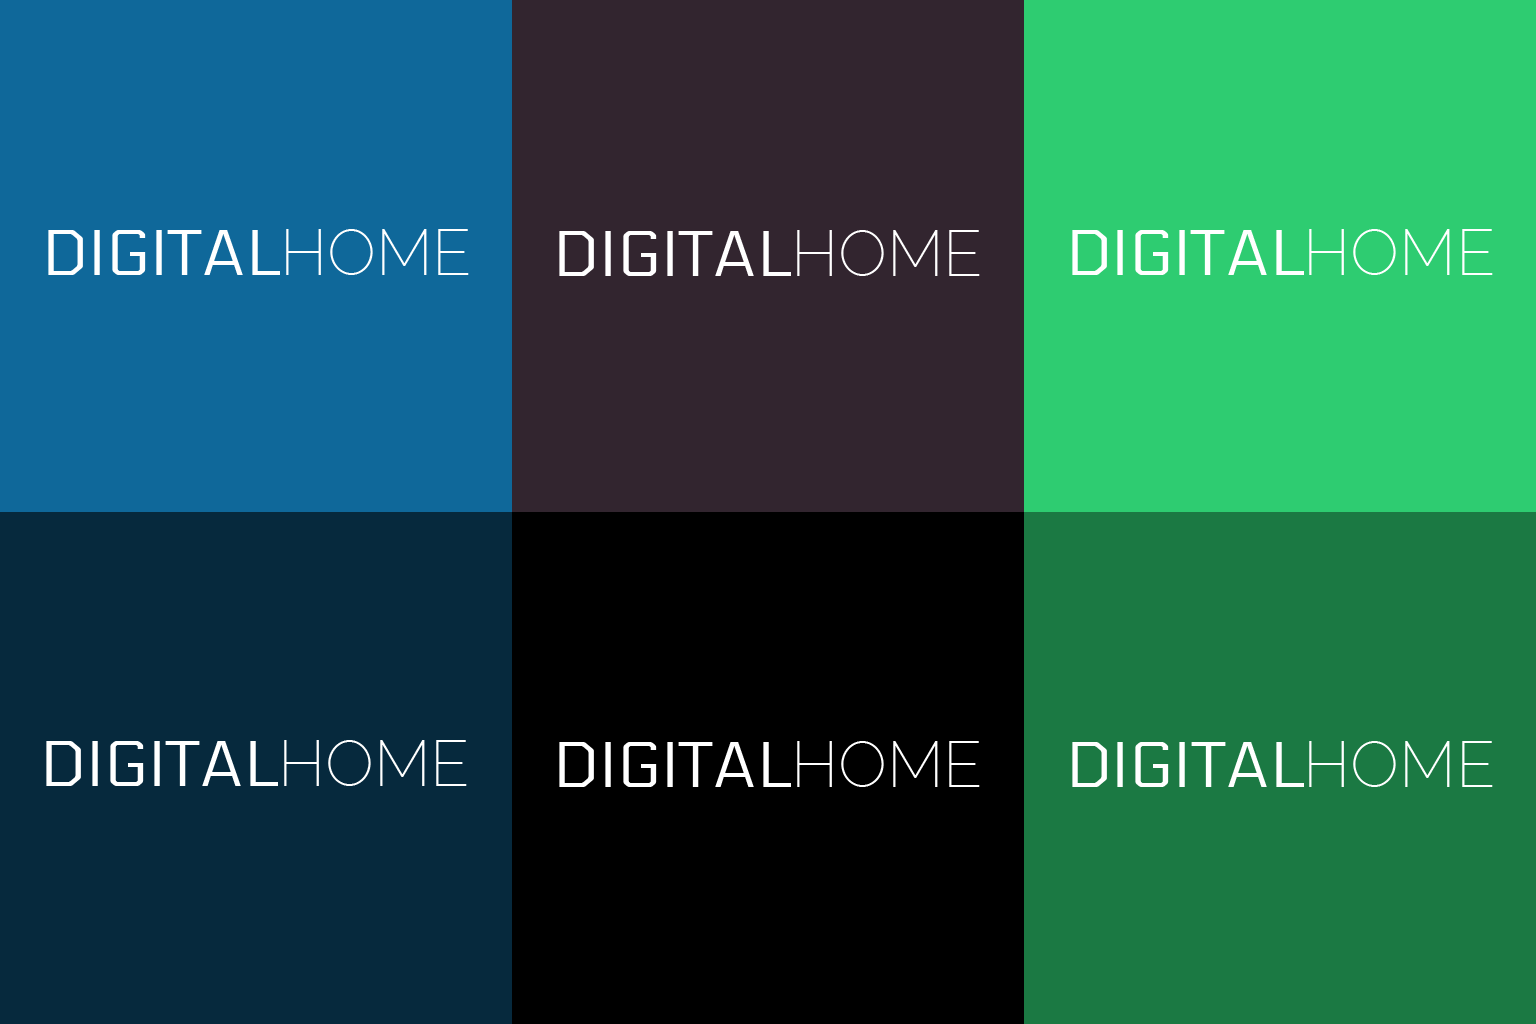
\includegraphics[width=\textwidth]{./img/zeitg_farbschema1.png}
	\caption{Das Farbschema des zeitgemäßen Ansatzes.}
	\label{zeitg:farbschema}
\end{figure}

Für den zeitgemäßen Ansatz wurde auf ein Monochromatisches Farbschema gesetzt, wie in Abbildung \ref{zeitg:farbschema} zu sehen. Blau und Schwarz sind Hauptfarben des Designs, Grün dient als alternative zu Blau.
Blau kommt aufgrund seiner Assoziation mit Technik und Intelligenz zum Einsatz. Die Farbe soll bei den Nutzern Vertrauen zur Seriösität des Unternehmens herstellen. Der Einsatz eines simplen Farbschemas ist vor allem der Bildlastigkeit des Designs zu verschulden.
Alle Farben sind als Pastellfarben auf eine gute Lesbarkeit ausgelegt. Ebenso wird die Webseite dadurch ruhiger und wirkt weniger Aufdringlich. Der Stresslevel wird reduziert.
Das alternative Farbschema ist ein völlig anderer Ansatz und soll trotz des technischen Konzepts ein Bezug zur Natur hergestellt werden. Der Nutzer soll hiermit eine Natürlichkeit bzw. Selbstverständlichkeit der Digitalisierung als Teil der Natur assoziieren.

\subsection{Typographische Gestaltung}
Für Überschriften und Texte wird ausschließlich auf die Font Familie Raleway zurückgegriffen. Aus dieser Familie kommen die Schriftbreiten 100 - 300 zum Einsatz, die unter Light/Thin geführt werden. Raleway bezeichnet sich selbst als Humanist-Sans. Dieser Teil der Font-Familie hat jedoch auch stilistische Eigenschaften einer Geometric-Sans Font, welche in Architektur und Wissenschaft sehr beliebt sind. Zwischen diesen beiden Typen liegen die Transitional-Sans. Diese sind gut mit den Themen Technologie und Wirtschaft zu verbinden. Architektur und Technologie sind eben jene zwei Kernbereiche der DigitalHome Idee, weshalb sich diese Font letzlich so gut eignet.
Auch in den anderen Ansätzen kommt diese Schriftart zum Einsatz. Vgl. Kapitel \ref{typo_inno} und \ref{chapter:mini:typo}.

\subsection{Strukturanalyse der Seite}\label{zeitg:struktur}
Strukturell ist dieser Ansatz recht konservativ mit einer Navigation am oberen Bildschirmrand, einem großen Blickfänger darunter und unter diesem der Inhaltsbereich im Kachel-Design. (Siehe Abbildungen \ref{zeitg:struktur1} und \ref{zeitg:struktur2})
Auf dem Blickfänger bzw. Titelbild ist das Logo mit dem Firmenname gut Sichtbar platziert, sowie eine Unterüberschrift direkt darunter. Zur besseren Lesbarkeit sind beide Blöcke durch Whitespace getrennt und haben einen Innenabstand von 1.5rem auf 16px normalisiert. Der Logo Block und die Unterüberschrift haben einen Abstand von 32px zueinander.

\begin{figure} [hp]
	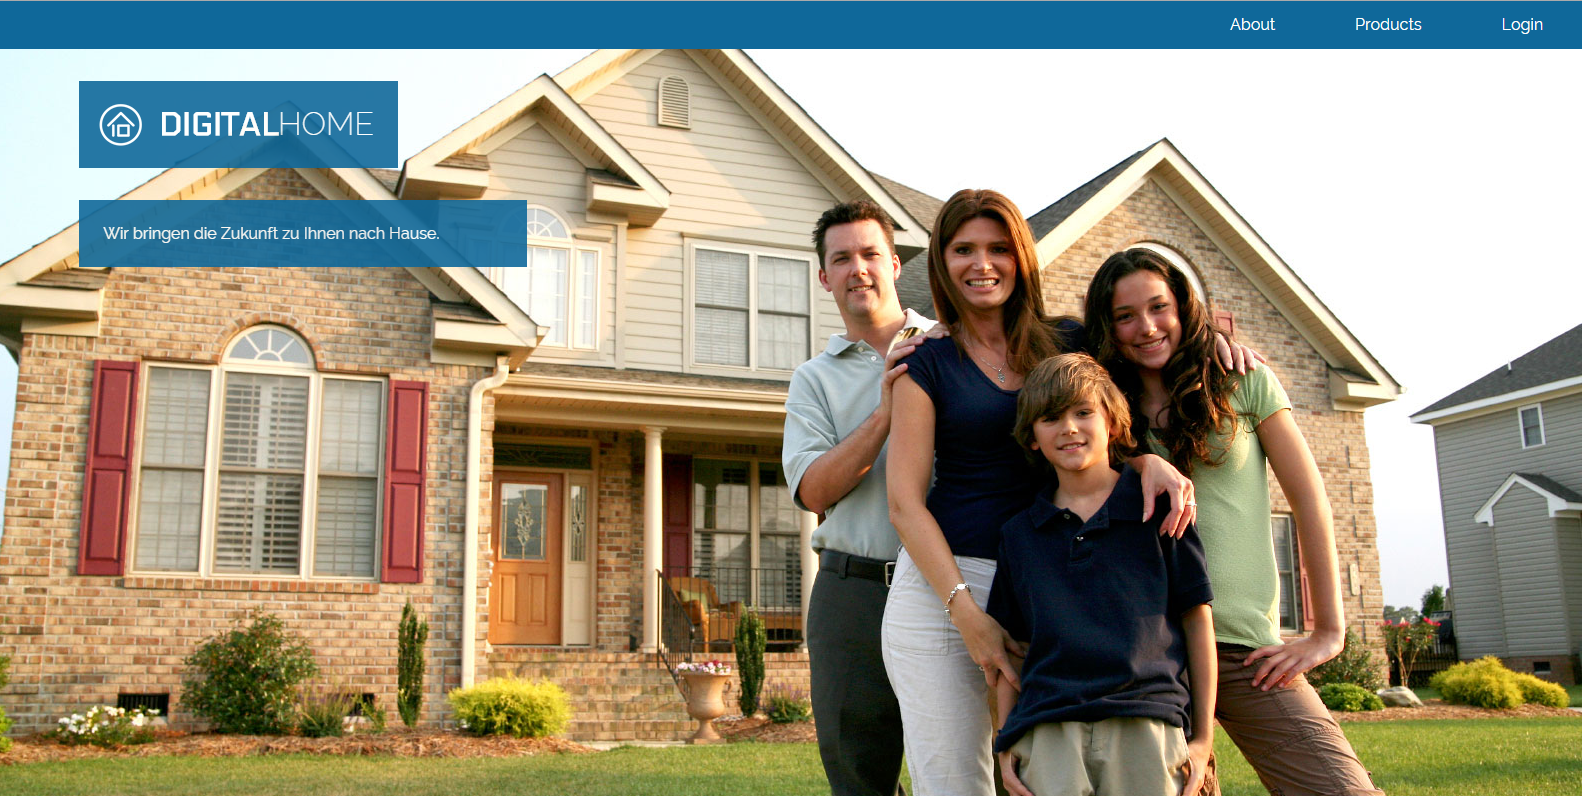
\includegraphics[width=\textwidth]{./img/zeitg_struktur1.png}
	\caption{Startseite im Programmierten Design. Navigation und Titelbild.}
	\label{zeitg:struktur1}
\end{figure}

\begin{figure} [hp]
	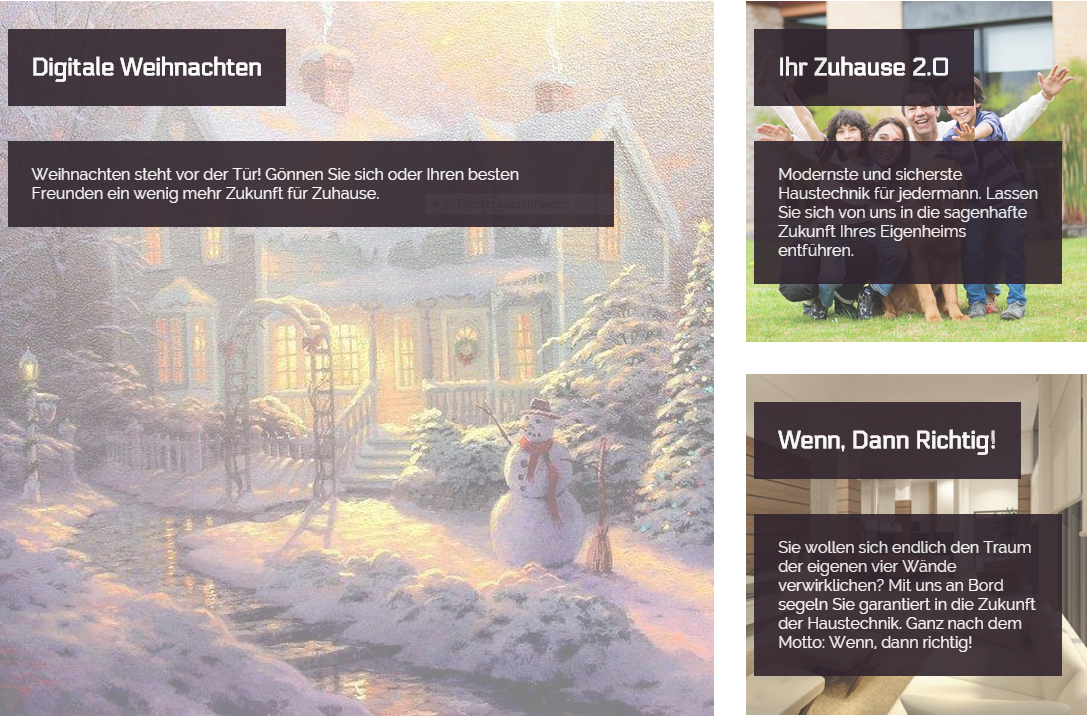
\includegraphics[width=\textwidth]{./img/zeitg_struktur2.png}
	\caption{Inhaltsbereich im programmierten Design des zeitgemäßen Ansatzes. Kacheldesign zum Darstellen des Inhalts.}
	\label{zeitg:struktur2}
\end{figure}

Um Botschaften zum Nutzer zu übertragen werden in diesem Design größtenteils Bilder verwendet, wie auch an dem großen Titelbild in Abbildung \ref{zeitg:struktur1} zu sehen ist. Transparenz der Schriftblöcke erleichtert das Erkennen der Bilder im Hintergrund. (Zu sehen in Abbildung \ref{zeitg:struktur2}).
Das Kachel-System in diesem Design basiert auf einem Grid-System mit einer Spaltenbreite von genau 320px und einem Spaltenabstand von 32px. Das System ist darüber hinaus mobil optimiert und folgt dem Responsive Webdesign Principle\footcite[vgl.][]{alistapart:rwd}. Anders als im allgemeinen Konsens arbeitet das System allerdings nach dem Adaptive Design Principle, welches ein bestandteil des RWD darstellt. Dabei gibt es CSS-Breakpoints für bestimmte definierte größen, wodurch das Design auch auf mobilen Geräten gut präsentiert wird. Wenn auch angemerkt werden muss, dass dieses Prinzip nicht derart flexibel ist wie ein Fluid-Design.
Zur besseren Hervorhebung und differenzierung einzelner Inhaltsblöcke gibt es verschiedene Arten von Kacheln. Standard sind hier die rechteckigen Kacheln der größe 320px. Kacheln mit der Eigenschaft \lstinline{~="featured"} werden in doppelter Größe in Höhe als auch Breite dargestellt. Die Eigenschaft \lstinline{~="extra"} verleiht der Kachel eine doppelte Breite.
Auf mobilen Endgeräten werden alle Kacheln auf Standardgröße reduziert sowie in einer einzigen Spalte angezeigt. Außerdem wird das Menü unter dem großen Bildbereich positioniert (Siehe Abbildung \ref{zeitg:struktur3}, derart, dass bei jeder Bildschirmgröße der Anfang des Menüs zu erkennen ist.

\begin{figure} [hp]
	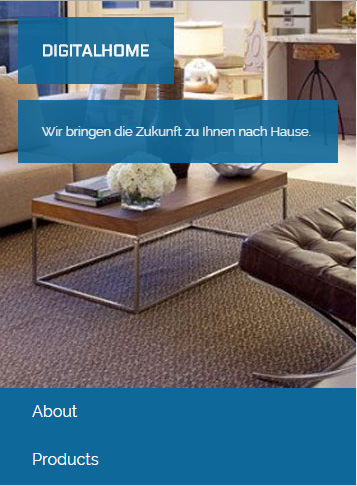
\includegraphics[width=0.5\textwidth]{./img/zeitg_struktur3.png}
	\caption{Startseite im Programmierten Design in der mobilen Ansicht. Navigation unter dem großen Bildbereich positioniert.}
	\label{zeitg:struktur3}
\end{figure}